\chapter{Introduction}

\dictum[Теодо́сій Григо́рович Добжа́нський (Theodosius
Dobzhansky)\footnotemark]{Nothing in biology makes sense […]}
\footnotetext{\citet{Dobzhansky:1973}}

\section{The central dogma}

% <<<
At the core of every living being is its genetic inheritance. The genetic
inheritance is what is being passed down from parents to their offspring, and
contains a blueprint detailing how to construct a new individual from a single
cell in a process called \define{embryogenesis}. This genetic inheritance is
physically present in the form of \dna in almost every living cell.\footnote{And
to some extent in non-living particles called \define{viruses}.}

As a medium of information storage, \dna is complemented by two other types of
molecules in the cell that, respectively, carry out the instructions encoded in
the \dna by performing specific biochemical functions, and serve as an
intermediary between information storage and execution. The intermediaries,
which are called \define{\rna}, copy out specific parts of the complete
instructions from the \dna and carry them to factories which translate the
instructions into highly specialised machines. These machines are called
\define{proteins}. The \define{central dogma of molecular biology} states that
information is thus transmitted from \dna to \rna, and from \rna to proteins,
but never from proteins back to \rna or \dna (\cref{fig:central-dogma})
\citep{Crick:1958,Crick:1970}. When first published, the central dogma concisely
summarised the available evidence at the time. Now, more than half a century
later, this still largely holds true.

\textfig{central-dogma}{body}{0.75\textwidth}
    {The central dogma of molecular biology.}{The solid arrows represent
    observed transfers of information; the dashed arrows represent what
    \citet{Crick:1970} referred to as “potential” transfers; today we know that
    the transfer \(\text{\rna}\rightarrow\text{\dna}\) does in fact occur under
    certain circumstances; the transfer \(\text{\dna}\rightarrow\text{protein}\)
    has still not been observed. Notably, the \emph{absent} transfers in the
    original publication are still considered largely non-existent.}

The very high-level view of the central dogma was complemented by a detailed
mechanistic description over the years, and the efforts to fill in all the
details are still ongoing. In this thesis I will present the results of my
exploration of one minute aspect concerning the translation of \rna into
proteins. To better explain how it fits into the general picture of the central
dogma, we first need to understand its leading actors and their interplay. The
three main roles in the central dogma are fulfilled by \dna, \rna and proteins,
respectively, and we are now going to take a look at all of them in turn.
% >>>

\subsection{\abbr{dna}}

% <<<
\dna consists of a long chain of \define[{\defineword{nucleotide} molecule
consisting of a ribose, one or more phosphate groups and a nucleobase (example:
cytidine monophosphate, a nucleotide of cytosine)\footnotemark\\%
\marginfig{nucleotide}}]{nucleotides}\footnotetext{Figure adapted from
\url{https://commons.wikimedia.org/w/index.php?title=File:Nucleotides_1.svg&oldid=128814238}}.
The chemical structure of nucleotides enables them to polymerise into long,
relatively stable chains. \dna is made up of nucleotide monomers, consisting of
one or more phosphate groups coupled to a \define[\defineword{nucleoside}
nucleobase coupled to a ribose]{nucleoside}, each of which contains any of four
different types of \define{nucleobases}: adenine (\nA), cytosine (\nC), guanine
(\nG) and thymine (\nT). Thus, \dna can be thought of as a long string of four
different letters, and that is indeed how it is often represented. Text is
written from left to right in Western cultures. By convention, \dna is written
from \fivep to \threep. The numbers refer to the numbering of the carbon atoms
in each nucleotide’s ribose, with the \threep carbon atom forming a covalent
bond with the phosphate of the next nucleotide, which is itself attached to the
\fivep carbon of its ribose. In this way, a \fivep \ce C atom is exposed at one
end of the chain, and a \threep \ce C is exposed at the other.

\dna is present in the cell in the form of double-stranded helices: each \dna
molecule consists of two paired chains, wound tightly around each other, with
the bases on each chain pairing up such that every \nA on one chain is paired
with a \nT on the other, and each \nC is paired with a \nG. This striking
symmetry is known as Watson–Crick base pairing, after its discoverers
\citep{Watson:1953}. Thus, \dna is made up of two complementary strands,
redundantly holding the genetic information. This redundancy is used in \dna
copying (which occurs at every cell division, and is the mechanism by which
genetic information is passed from one cell to its offspring) to synthesise two
newly formed \dna molecules, of which each contains one strand of the parent
\dna molecule (\define{semiconservative replication}) \citep{Meselson:1958}.

\todo[inline]{Double helix structure with one part annotated as a gene; histones?}

The information on the \dna is not stored in one consecutive piece. Rather, \dna
consists of relatively short stretches encoding a specific function, separated
by long stretches that do not directly encode any function. The “function” is
what is transmitted, as per the central dogma, to \rna and, in many cases, on to
proteins. Such self-contained, functional stretches are called
\define[\defineword{gene} self-contained stretch of \abbr{dna} that is
transcribed to perform a function]{genes}. To perform its function, a gene has
to be transcribed into a catalytically active form, the \rna.\todo[ref]{Human Genome Project}
% >>>

\subsection{\abbr{rna}}

% <<<
\rna is the product of transcription of a gene from \dna. Unlike the latter,
\rna is created as a single strand. This has two consequences: First, \rna is
much less stable than \dna, and slowly degrades. \rna thus has a finite
life-time, and the pool of \rna must be replenished by continuous transcription.
Second, single-stranded ribonucleic acid spontaneously changes its spatial
conformation by forming Watson--Crick base pairs between nucleotides in its own
sequence, where this is \define[\defineword{steric effect} atoms occupy discrete
space and cannot overlap]{sterically} possible (i.e.\ where forming such a bond
does not require bending the chain too much to “snap” it). The resulting
structure can have functional consequences for the \rna. Because the structure
is determined by, and exists on a higher level than the sequence identity of the
\rna, it is called \define{secondary structure}.

Another difference between \dna and \rna is the use of slightly different
nucleobases: instead of \nT, \rna uses \nU (uracil), which, like \nT, base-pairs
with \nA. Despite the fact that the genetic information is encoded in virtually
the same way in \dna and \rna, transcription of \dna into \rna requires a
complex machinery. The core of this machinery is a complex enzyme called an
\define{\rna polymerase}. In eukaryotes, three different, evolutionarily related
\rna polymerases (\pol1, \pol2 and \pol3) are responsible for transcribing
different types of \rna.

\rna performs numerous different functions, but one very important subcategory
of \rna does not perform any function on its own; rather, it is an intermediary
between the genetic information on the \dna and the final protein product, which
in turn performs cellular functions. This class of \rna is called \mrna.
\mrna[s] are the product of the transcription of protein-coding genes by \pol2.
By contrast, \rna[s] which are not protein-coding are denoted as \ncrna.
Transcription of \mrna requires an exquisite control, and many different \tf[s]
are known to regulate different genes in different cellular conditions. This
results in different \mrna genes being transcribed at highly different levels,
leading to several orders of magnitude of difference in \mrna abundance. Even
more strikingly, the same \mrna can be transcribed at different levels under
different conditions. \mrna is further processed in several steps before the
mature \mrna is exported from the cell’s nucleus into the cytoplasm, where it is
translated into proteins, and, over time, decays. Taken together, this leads to
very differentiated \mrna profiles under different conditions, which imbue the
cells with a unique phenotype. This forms the basis of cellular differentiation
into different cell types and tissues in multicellular eukaryotes.\todo{Introns?
Alternative splicing?}\todo[ref]{Berthelot, Ule}
% >>>

\subsection{Proteins}

% <<<
Proteins, finally, are the main effectors of cell function. Like \dna and \rna,
they consist of chains of smaller molecules, so-called
\define[{\defineword{amino acid} molecule consisting of an amino–carboxyl
backbone and a specific side-chain (example: valine)\\%
\marginfig{amino-acid}}]{amino acids}, which are strung together to form
\define{polypeptides}. Each amino acid is a small molecule with unique
properties which, jointly, shape the function of the final protein. Individual
amino acids are strung together in a chemical reaction that links a carboxyl
group covalently with an amino group on the next amino acid to form a
\define[\defineword{peptide bond} a covalent bond formed between a carboxyl and
an amino group: \ce{COOH + NH2 -> CO-NH + H2O}]{peptide bond}
\citep{Alberts:2002}. Polypeptides, like many \rna[s], form secondary structures
via non-covalent bonds between amino acids, which are a function of the amino
acid sequence. Beyond this, proteins form even higher order three-dimensional
conformations called tertiary structures. When multiple proteins aggregate into
a complex consisting of several subunits, we speak of quarternary structure.

All these different levels of spatial organisation of proteins lead to the
creation of highly complex structures from originally one-dimensional chains. It
is their intricate structure which allows them to perform precise tasks in the
cell. Because they are the work horses of the cells, proteins are highly
abundant, with some proteins being present million-fold at any given moment
\citep{Milo:2013}. This is only possible because a single gene is transcribed
multiple times at once, and each resulting \mrna can be translated several
times, and simultaneously, before being degraded. The path
\(\text{\dna}\rightarrow\text{\rna}\rightarrow\text{protein}\) thus facilitates
an amplification from a single gene copy to many orders of magnitudes more
copies of the resulting protein. Despite the fact that multiple protein copies
can be created from a single \mrna molecule, and that the number varies from
transcript to transcript, protein abundance is predominantly determined by the
abundance of \mrna[s] \citep{Li:2014,Jovanovic:2015,Csardi:2014}.
% >>>

\section{Transcription \& translation}

\subsection{Transcription}

% <<<
As mentioned, three different polymerases are responsible for transcribing
nuclear \dna into different types of \rna. The precise ways in which the
different polymerases transcribe genes into their \rna products differ but the
fundamental aspects of transcription are similar. In all cases, a
\define[\defineword{motif} pattern describing a family of short sequences which,
though variable, have some degree of similarity]{motif} in the \dna sequence
initiates binding of a number of \tf proteins to the \dna. Such motifs, called
\define{promoters}, are found in the immediate vicinity of the \tss of their
target genes --- either upstream of the \tss or following closely after it,
inside the gene body. Once the \tf[s] have bound to the \dna on top of the \tss,
a polymerase attaches to the \dna and is held in place by the \tf[s].
Subsequently, the polymerase pries the double strand apart and starts
synthesising a new strand of \rna which pairs complementary with one of the
strands on the \dna (the \define{template strand}). The new \rna[’s] sequence is
thus identical to the other \dna strand (the \define{coding strand}). The \rna
is produced in the direction \fivep--\threep, implying that the template strand
is read in the direction \threep--\fivep during transcription. Once the first
few nucleotides of the \rna have been synthesised, the polymerase disassociates
from the \tf proteins, and the polymerase starts moving along the gene body,
transcribing it as it goes (this may require the presence of other \tf[s] called
\define{activators}, which are recruited by \define{enhancer} motifs elsewhere
on the \dna).

\todo[inline]{Figure: Transcription}
\todo[inline]{Histone marks and regulation}
% >>>

\subsection{The genetic code}

% <<<
The process by which proteins are created from \mrna transcripts is more complex
than the 1:1 transcription of \dna into \rna, which after all use a common
alphabet to encode the information they carry. By contrast, the
\define{translation} of \mrna transcripts into proteins requires a code to
interpret the genetic information.

There are \num{20} different amino acids that are encoded by just \num{4}
different nucleotides. To allow this, several nucleotides must be combined to
form a larger unit coding for an amino acid. In the universal \define{genetic
code}, shared by all known species, this is accomplished by grouping three
consecutive nucleotides together to form non-overlapping \define{codons} along
the \mrna. This results in \(4^3 = 64\) possible codons, vastly more than there
are amino acids. As a consequence, the genetic code is \define{degenerate}: most
amino acids can be encoded by more than a single codon.

\begin{table}[!ht]
    \centering
    \def\s{\footnotesize stop}
    \def\h#1#2{\multicolumn{1}{#1}{\abbrsc{#2}}}
    \begin{tabu} to \textwidth {@{}
            >{\collectcell\codon}l<{\endcollectcell}
            >{\collectcell\anticodon}l<{\endcollectcell}
            l @{\qquad}
            >{\collectcell\codon}l<{\endcollectcell}
            >{\collectcell\anticodon}l<{\endcollectcell}
            l @{\qquad}
            >{\collectcell\codon}l<{\endcollectcell}
            >{\collectcell\anticodon}l<{\endcollectcell}
            l @{\qquad}
            >{\collectcell\codon}l<{\endcollectcell}
            >{\collectcell\anticodon}l<{\endcollectcell}
            l @{}}
        \toprule
        % Nasty, hand-coded length values.
        \noalign{\vskip-4pt}
        \h{@{}l}{C} & \h{l}{A} & \h{l}{AA} &
        \h{@{}l}{C} & \h{l}{A} & \h{l}{AA} &
        \h{@{}l}{C} & \h{l}{A} & \h{l}{AA} &
        \h{@{}l}{C} & \h{l}{A} & \h{l@{}}{AA} \\[-2pt]
        \midrule
        UUU & AAA & Phe & UCU & AGA & Ser & UAU & AUA & Tyr & UGU & ACA & Cys \\
        UUC & GAA & Phe & UCC & GGA & Ser & UAC & GUA & Tyr & UGC & GCA & Cys \\
        UUA & UAA & Leu & UCA & UGA & Ser & UAA & UUA & \s  & UGA & UCA & \s \\
        UUG & CAA & Leu & UCG & CGA & Ser & UAG & CUA & \s  & UGG & CCA & Trp \\
        \addlinespace
        CUU & AAG & Leu & CCU & AGG & Pro & CAU & AUG & His & CGU & ACG & Arg \\
        CUC & GAG & Leu & CCC & GGG & Pro & CAC & GUG & His & CGC & GCG & Arg \\
        CUA & UAG & Leu & CCA & UGG & Pro & CAA & UUG & Gln & CGA & UCG & Arg \\
        CUG & CAG & Leu & CCG & CGG & Pro & CAG & CUG & Gln & CGG & CCG & Arg \\
        \addlinespace
        AUU & AAU & Ile & ACU & AGU & Thr & AAU & AUU & Asn & AGU & ACU & Ser \\
        AUC & GAU & Ile & ACC & GGU & Thr & AAC & GUU & Asn & AGC & GCU & Ser \\
        AUA & UAU & Ile & ACA & UGU & Thr & AAA & UUU & Lys & AGA & UCU & Arg \\
        AUG & CAU & Met & ACG & CGU & Thr & AAG & CUU & Lys & AGG & CCU & Arg \\
        \addlinespace
        GUU & AAC & Val & GCU & AGC & Ala & GAU & AUC & Asp & GGU & ACC & Gly \\
        GUC & GAC & Val & GCC & GGC & Ala & GAC & GUC & Asp & GGC & GCC & Gly \\
        GUA & UAC & Val & GCA & UGC & Ala & GAA & UUC & Glu & GGA & UCC & Gly \\
        GUG & CAC & Val & GCG & CGC & Ala & GAG & CUC & Glu & GGG & CCC & Gly \\
        \bottomrule
    \end{tabu}
    \tabcap{genetic-code}{The genetic code.}
        {Shown is each codon (“\abbrsc{C}”), its potential corresponding
        anticodon (“\abbrsc{A}”) and the three-letter abbreviation of the
        corresponding amino acid (“\abbrsc{AA}”). \codon{AUG}, in addition to
        encoding methionine, also signals the start of translation. Not all
        anticodons exist in all species. Each anticodon is the reverse
        complement of its corresponding codon (adapted from
        \citet{Dos_Reis:2004}).}
\end{table}

Codons furthermore serve as control points by defining where the translated
sequence on the \mrna starts and ends. The codon \codon{AUG}, in addition to
encoding the amino acid methionine, also marks the start of the coding sequence.
Three codons do not encode any amino acid, and instead signal the stop of
translation (\codon{UAA}, \codon{UAG}, \codon{UGA}). As a consequence, every
coding sequence starts with \codon{AUG}, ends with one of the stop codons, and
has a length divisible by \num{3}. \Cref{tab:genetic-code} contains a tabular
representation of the genetic code, which is valid, with only minor variations,
for all three domains of life.

During translation, individual codons on the \mrna transcript are successively
paired up with their matching amino acid. However, unlike in translation, this
pairing does not happen automatically. It requires an intermediate adapter
molecule acting as an interface between the codon and the amino acid.
% >>>

\subsection{Transfer \abbr{rna}}

% <<<
Individual codons are translated into their corresponding amino acid with the
aid of adapter molecules carrying a specific amino acid, and which recognise the
matching codon. This codon recognition is possible because the adapter molecules
are themselves \abbr{rna}s, and the codon is matched via complementary base
pairing of a part of the \rna sequence termed the \define{anticodon}. These
adapter molecules are called \trna.

\trna[s]\marginpar{
    \vspace{-12ex}% Necessary to fix figure going over bottom of page.
    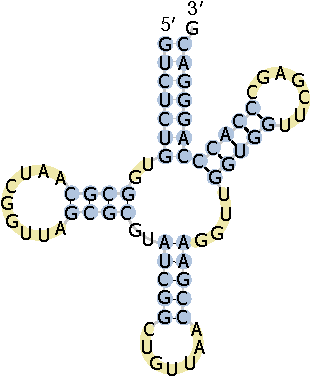
\includegraphics[width=\marginparwidth]{trna-asn}
    \figcapof{trna-asn}{\(\text{\abbr{trna}}^{\text{Asn}}\) secondary
    structure.}{ The \abbr{trna} carries the anticodon \anticodon{GUU} in the
    middle of the anticodon loop, highlighted in \tertiaryname{}. The D loop and
    T loop are shown in \primaryname{} and \secondaryname{}. Structure predicted
    by \name{COVE} \citep{Eddy:1994}, rendered by \name{PseudoViewer 3}
    \citep{Byun:2009} and manually edited.}
}
form secondary structures with a shape that vaguely resembles a
cloverleaf, consisting of a stem and three loops: the \define{D loop} (also
known as \define{DHU loop} because it contains the modified nucleobase
dihydrouridine), the \define{T loop} (or \define{TΨC loop}, because it contains
the nucleobase pseudouridine) and the \define{anticodon loop}. The latter
carries three nucleotides in its centre that pair with a specific codon --- the
anticodon \citep{Rich:1978,Schimmel:1979}.

To avoid confusion between codons and anticodons, codons in this thesis will
always be typeset as \fwdstrand{\codon{CAU}}, and anticodons (which are the
reverse complements of codons) will always be typeset as
\fwdstrand{\anticodon{AUG}}. The directionality is indicated here to clarify the
direction in which a codon pairs with its anticodon; it will generally be
omitted in the remainder of the text.

\todo[inline]{mRNA--tRNA pairing figure here, or later?}

\trna[s] are encoded by small genes, around \SIrange{70}{90}{bp} in length.
Their transcription is driven by \pol3. Transcription initiation for \pol3 can
take various forms for different types of genes. \trna genes perform so-called
\define{class~\abbrsc{II}} \pol3 transcription initiation. Unlike for
protein-coding genes, whose promoters lie upstream of the actual gene body, the
promoter is found \emph{inside} a \trna gene, in two disjoint, strongly
conserved regions called the \define{A box} and \define{B box}, respectively.
The A box starts about \SI{10}{bp} downstream from the \tss, whereas the B box
can be found at a variable distance of about \SIrange{30}{60}{bp} downstream
from the A box. \trna transcription is initiated when the transcription factor
\tfiiic binds to both motifs. This leads to the binding of the \pol3 recruitment
factor \tfiiib immediately upstream of the \trna gene. Subunits of \tfiiib, in
particular as the \tbp, bind to upstream motifs of the \trna, which vary
strongly across evolution, but whose presence is nevertheless crucial for the
initiation of transcription \citep{Palida:1993,White:1992}. Binding of \tfiiib
in turn leads to the association of \pol3 with the gene body, and the initiation
of transcription. \tfiiic is now no longer required and disassociates from the
gene locus. \tfiiib remains bound and can lead to repeated transcription
re-initialisation. Transcription stops when \pol3 encounters a short \nT repeat
downstream of the \trna gene (see \cref{fig:trna-gene})
\citep{White:1998,Dieci:2007}.

\textfig{trna-gene}{body}{\textwidth}{\abbr{trna} gene transcription}
    {immediately before \pol3 is recruited. The A and B box are highlighted in
    \primaryname{} and \secondaryname{}, respectively. The colours show the
    correspondence of these regions with the loops shown in \cref{fig:trna-asn}.
    The \seq{TATA} motif is a non-representative example of upstream motifs
    which are recognised by \abbr{tfiiib}. Diagram is not to scale.}

\trna genes exist in abundant gene copies. In the latest reference genome of
\mmu, \abbr{grcm38} \citep{Church:2009}, \num{432} different \trna genes are
annotated, encoding \num{50} different anticodons. \trna genes carrying the same
anticodon form an \define{anticodon isoacceptor family}. \trna genes for the
same amino acid form an \define{amino acid isotype}.

The numbers of \trna genes and anticodon isoacceptor families above exclude
\trna[s] for the amino acid selenocysteine, which is not part of the standard
genetic code, and which was consequently excluded from the subsequent analysis.
Selenocysteine is generally not included in analyses with a focus on codons in
the published literature, as it requires \define{translational recoding}, an
altogether different translation mechanism. Furthermore, the prevalence of
proteins incorporating selenocysteine is very small \citep{Reeves:2009}.
Although this does not mean that selenocysteine is biologically irrelevant, it
means that we can safely ignore its effect for transcriptome-wide studies of
codons and anticodon abundance.

After transcription, the newly formed precursor \trna transcript undergoes
processing to form a mature \trna. As for all types of \rna, this happens while
the precursor \trna is still in the nucleus of the cell, before it is then
exported into the cytoplasm where it performs its function.

The postprocessing of the \trna is required to ensure that the \trna folds into
its correct spatial structure, can be associated with an amino acid, and
recognises its target codons. It also serves as a quality control mechanism: in
the case where transcription introduced errors into the \trna sequence, no
postprocessing can occur, which prevents the subsequent export of the \trna from
the nucleus. This include splicing out introns from the \trna gene (although
this occurs rarely, as most \trna[s] have no introns) and cleavage of \fivep
upstream sequence elements \citep{Alberts:2002,Berg:2002}.

Another important processing step is the substitution of the \threep-most bases
by \fwdstrand{\seq{CCA}}, which will subsequently server as an anchor for the
attachment of an amino acid. Furthermore, several nucleotides of the \trna are
replaced by “unusual” nucleosides. Some of these are shown in
\cref{fig:trna-asn}. In particular, dihydrouridine (\seq D) replaces several
uridine\footnote{the nucleoside of uracil} nucleosides in the D loop, and
pseudouridine (\seq Ψ) replaces a uridine in the T loop. In total, about
\num{10} per cent of all nucleosides are modified in this manner, and over
\num{70} different types of base modifications are known to occur in \trna
\citep{Limbach:1994,Dalluge:1997,Alberts:2002}. Crucially, the \fivep base of
the anticodon also undergoes modification in this manner, and this plays an
important part in \define{wobble base pairing}.

\subsubsection{Wobble base pairing}

As \cref{tab:genetic-code} shows, there are \num{61} different codons. However,
not all of these have corresponding anticodon \trna[s] --- as mentioned, there
are only \num{50} different anticodon isoacceptors in \mmu; for example,
\codon{CUC} codes for leucine, yet there is no matching \anticodon{GAG}
anticodon \trna. Instead, a \codon{CUC} codon can pair with a \trna carrying a
\anticodon{AAG} anticodon. The mismatching \threep base of the codon is known as
the \define{wobble position} due to its ability to “wobble” around during codon
recognition, and thus being able to form hydrogen bonds which would not be
sterically possible under normal conditions. Unlike the first two bases of the
codon, the third base thus does not require a strict Watson--Crick match.

However, even under the thus relaxed steric constraints, \nA does not pair with
\nC. In order for the \anticodon{AAG} isoacceptor \trna[s] to recognise the
\codon{CUC} codon, it therefore has to have undergone a base modification of its
wobble base. Indeed this is what happens, with the adenosine (the nucleoside of
adenine) aat the \fivep position being replaced by inosine (the nucleoside of
hypoxanthine, short \nI). \nI is able to pair with \nA, \nC and \nU when it is
in the wobble position, and the modified \anticodon{IAG} is thus able to decode
\codon{CUC} \citep{Crick:1966,Murphy:2004}. Despite the existence and importance
of these base modifications to the anticodon, I will continue using the
genomically encoded anticodon notation rather than the anticodon after base
modification --- in other words, I will generally write \anticodon{AAG}, not
\anticodon{IAG}, by general convention. \Cref{tab:wobble} lists the possible
wobble base pairings.

\begin{table}[!ht]
    \centering
    \begin{tabular}{@{}ll@{}}
        \toprule
        Codon & Anticodon \\
        \midrule
        \nC & \nG \\
        \nG & \nC, \nU \\
        \nU & \nA, \nG \\
        \nI & \nA, \nC, \nU \\
        \bottomrule
    \end{tabular}
    \tabcap{wobble}{Simplified wobble base pairing rules.}{This table is based
    on a prediction by \citet{Crick:1966}. In practice, more pairings are
    possible (though most are uncommon), and there exist several other modified
    bases with unique pairing properties.}
\end{table}

\subsubsection{Amino acid activation}

Once mature, the \trna is exported from the nucleus into the cytosol to aid in
\mrna translation. We have seen how a \trna recognises a specific codon via
interaction with its anticodon. This still leaves the question of how the \trna
interacts with its target amino acid. In fact, so far the \trna is “empty” ---
not bound to any amino acid. It needs to be “charged” with an amino acid before
it can act as an adapter. Conversely, we could say that amino acids need to be
\define{activated} by being coupled to a transfer molecule, which makes them
suitable to be used in protein synthesis. This activation is handled by the
protein \define{aminoacyl-\trna synthetase}.

Aminoacyl-\trna synthetases are enzymes that take a target amino acid and
covalently attach it to the \threep end of a matching \trna. This implies that
aminoacyl synthetases need to be able to recognise the correct binding partners.
In most species, there are \num{20} different aminoacyl-\trna synthetases ---
one per amino acid. Each of them is responsible for charging all \trna[s] for a
given amino acid isotype. The aminoacyl-\trna synthetase recognises a matching
\trna by probing for several sequence features, including the acceptor stem, the
anticodon and a specific base immediately adjacent to the \threep end of the
\trna. Once it has associated with an amino acid and its matching \trna, it
catalyses the binding of the amino acid to the \threep adenosine of the \trna,
to form an aminoacyl-\trna
\citep{Schimmel:1979,Schimmel:1993,Ibba:2000,Alberts:2002}.

Thus loaded with an amino acid, the aminoacyl-\trna is now free to participate
in the translation reaction, wherein it will bind to a matching codon and give
up its attached amino acid. This will leave it once more empty but otherwise
intact, so that it can be recharged immediately by another aminoacyl-\trna
synthetase. \trna molecules are thus repeatedly reused until the molecular
structure degrades, and gets recycled by the cell.
% >>>

\subsection{Translation}

% <<<
The translation of \mrna into proteins is assisted by a special apparatus called
the \define{ribosome}. Ribosomes are large complexes of proteins and \rrna,
forming two subunits. In eukaryotes, these subunits are the 40S and 60S subunit,
respectively. During translation initiation, the 40S subunit scans along an
\mrna transcript until it finds a signal sequence surrounding a start codon
\citep{Kozak:2002}. There it is joined by the 60S subunit. The assembled
ribosome then pulls the \mrna through a channel in its structure and
progressively translates the codons on the \mrna into amino acids, which are
chained together to form a nascent polypeptide chain.
% >>>

\section{\abbr{rnaseq} for the study of gene expression}

\section{\abbr{chipseq}}

\subsection{\abbr{chipseq} quantifies \abbr{trna} gene expression}

\section{Mouse development as a model system}

\section{Quantifying codon usage and anticodon abundance}

\todo[inline]{Description of the goals of the thesis}

We have seen how the genetic code defines the interface between \mrna and
proteins, and how \trna[s] are the physical link between the codons on the one
hand and the amino acids on the other hand. As the abundance of different \mrna
transcripts varies with the cell state, so does the number of different codons
that are used by these transcripts. This immediately suggests that the variable
demand of codons to be decoded needs to be met, in some way, by a supply of
\trna molecules carrying matching anticodons. In this thesis, I am going to
explore this supply--demand relationship between codons and anticodons by
investigating the abundance of \trna[s] in cells and its relationship to the
demand of codons in the \mrna transcriptome.

Throughout this thesis I am going to use several related measures:

\begin{enumerate}
    \item codon usage,
    \item \rcu,
    \item anticodon abundance and
    \item \raa.
\end{enumerate}

The \define{codon usage} of a codon is the frequency with which this codon
occurs in a given transcriptome. This is either the raw number of occurrences in
the transcripts under consideration, or the number of occurrences, weighted by
the expression of each transcript.

The \define{anticodon abundance} of an anticodon is the amount of \trna
decoding a given anticodon, present in the cell at a given instance. Other
publications define the anticodon abundance in terms of \trna gene copy number;
however, in the context of this thesis, the anticodon abundance is usually
quantified by \trna gene expression, and is thus proportional to the number of
\trna molecules of each anticodon isoacceptor present in the cell.

The \define{\rcu} of a codon is that codon’s contribution to the amino acid it
codes for, relative to all other synonymous codons. The \rcu of all synonymous
codons sums to \num{1}.

The \define{\raa} of an anticodon is defined equivalently to the \rcu based on
the anticodon abundance. That is, the contribution of an anticodon to its amino
acid isotype, relative to the other anticodons in the same isotype.

In all of the above, I exclude the stop codons.

Several publications use the term \cub to describe divergence in codon usage
between different sets of genes within a genome, or differences between genomes.
The \cub is then equivalent either to the codon usage as defined in this thesis,
or the \rcu.

\section{Structure of this thesis}

\section{TO DOs}

\todo[inline]{\begin{enumerate}[noitemsep,nolistsep,leftmargin=*]
    \item Molecular and functional structure description of pol2 and pol3
    \item tRNA modification, (re)loading and degradation: life-cycle has impact
        on abundance, and thus on translation efficiency. We completely ignore
        this; but why can we do this?
    \item tAI, codon usage, codon usage bias, anticodon abundance bias
    \item Tiny bit about mouse embryonology
    \item Prior research/literature review of tRNA and codon usage, also outside
        mammals! Dittmar [2006]
\end{enumerate}}

\todo{Take intro from paper}

\subsection{Posttranscriptional modification}

In particular A-to-I conversion (deamination), which is relevant in tRNA gene
wobble base pairing!
% vim: fmr=<<<,>>>
